% THIS IS SIGPROC-SP.TEX - VERSION 3.1
% WORKS WITH V3.2SP OF ACM_PROC_ARTICLE-SP.CLS
% APRIL 2009
%
% It is an example file showing how to use the 'acm_proc_article-sp.cls' V3.2SP
% LaTeX2e document class file for Conference Proceedings submissions.
% ----------------------------------------------------------------------------------------------------------------
% This .tex file (and associated .cls V3.2SP) *DOES NOT* produce:
%       1) The Permission Statement
%       2) The Conference (location) Info information
%       3) The Copyright Line with ACM data
%       4) Page numbering
% ---------------------------------------------------------------------------------------------------------------
% It is an example which *does* use the .bib file (from which the .bbl file
% is produced).
% REMEMBER HOWEVER: After having produced the .bbl file,
% and prior to final submission,
% you need to 'insert'  your .bbl file into your source .tex file so as to provide
% ONE 'self-contained' source file.
%
% Questions regarding SIGS should be sent to
% Adrienne Griscti ---> griscti@acm.org
%
% Questions/suggestions regarding the guidelines, .tex and .cls files, etc. to
% Gerald Murray ---> murray@hq.acm.org
%
% For tracking purposes - this is V3.1SP - APRIL 2009

\documentclass{acm_proc_article-sp}

\usepackage{url}
\usepackage{listings}
\usepackage{graphicx}
\usepackage{fixltx2e}
\usepackage{moreverb}
\usepackage{fancyvrb}
\usepackage{csvsimple}
\begin{document}

\numberofauthors{2} 
\author{
\alignauthor
Ivan Oropeza\\
       \affaddr{Dept. of Computer Science}\\
       \affaddr{University of Texas at Austin}\\
\alignauthor
William Xie\\
       \affaddr{Dept. of Computer Science}\\
       \affaddr{University of Texas at Austin}\\
}

\title{Hidden Markov Models vs. Maximum Entropy Markov Models}


\maketitle
\section{Introduction}
A frequent problem in many disciplines is the challenge to do sequence labelling. DNA sequencing, video semantic analysis, and Part-Of-Speech tagging are just some examples where sequence labelling is the underlying problem that needs to be solved~\cite{dnaEx, videoEx, nlpEx}. In Natural Language Processing (NLP), Part-Of-Speech (POS) or lexical category tagging is an important problem because it serves as a stepping stone into solving more complex problems such as semantic analysis of sentences. The typical techniques applied to this problem are Hidden Markov Models (HMM), Maximum Entropy Markov Models (MEMM), and Conditional Random Fields (CRF). While CRFs are considered to be the state-of-the-art in POS tagging we want to compare the performance of the other models, HMM and MEMM. This paper is structured in the following way: first we provide a brief description of the datasets used in this investigation. Then, we discuss some of the differences between HMMs and MEMMs. Next, we explain how the training process works specifically for POS tagging. Finally, we compare the performance of HMMs vs MEMMs under similar circumstances.

\section{Datasets}
In this investigation we use two corpora. The first one is the Wall Street Journal (WSJ) corpus. The WSJ corpus is a collection of 2,499 articles collected in a span of three years from the Wall Street Journal. It has approximately 3 million words and was tagged by using statistically-based methods. This corpus has a total of 82 possible tags~cite{wsjCorpus}. Its range of topics is very narrow and thus it is reasonable to expect that the word choice distribution in the articles to be narrower than other corpora as well. Hence, we expect better performance when we test with this metric.

In addition to the WSJ corpus, we also use the Brown corpus. The Brown corpus is a manually tagged collection of 500 text documents sampled from 1961. It uses 36 POS tags and it is consolidated from various sources and from various topics such as fiction, press, and lore~\cite{brownCorpus}. Consequently, we expect that this corpus would represent a more general distribution on word choice than WSJ corpus. Therefore, we expect scores to be slightly lower than when using WSJ.

\begin{figure}[ht]
 \begin{Verbatim}[frame=single,framesep=5mm]
\[ He/PRP \]
tried/VBD to/TO ignore/VB 
\[ what/WP \]

\[ his/PRP\$ own/JJ common/JJ sense/NN \]
told/VBD 
\[ him/PRP \]
,/, but/CC 
\[ it/PRP \]

\[ was/VBD n't/RB possible/JJ \]
;/: ;/: 
\[ her/PRP$ motives/NNS \]
were/VBD too/RB blatant/JJ ./.

\end{Verbatim}
\caption{Example sentence from the Brown Corpus~\cite{brownCorpus} \label{brownExample}}
\end{figure}

\section{HMM vs. MEM,}
A HMM is generative model for the joint distribution of states and observations. It follows a Markovian assumptions. The Markov assumption restricts the transitions between states to be dependent only on the immediate past~\cite{nlpBook}. On the other hand, MEMM is discriminative since it models the conditional probability of the state given the observation. 

An MEMM is an enhancement on the Maximum Entropy model, also known as a multinomial regression model which in turn attempts to do classification by making the fewest number of assumptions. Figure \ref{hmmVmemm} shows the pictorial differences between both graphical models. The added benefit of MEMMs over HMMs is that MEMMs are not limited to only modelling two aspects: $P( S_i | P_{i-1} )$ and $P( O_i | S_i )$. Instead, MEMMs consider information derived directly from features applied on the observation in addition to the previous state knowledge. For example, capitalization often occurs with Nouns and specific suffixes such as "ed" and "ing" tend to be associated with Verbs are some useful features that can not be modelled by an HMM but can be modelled by an MEMM. Moreover, the typical algorithm used to solve the decoding problem in an HMM can be trivially modified to solve the decoding problem in an MEMM without additional overhead~\cite{nlpBook}.
\begin{figure}[ht]
\centering
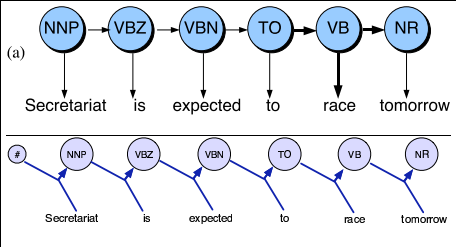
\includegraphics[width=80mm]{figures/memm.png}
\caption{Hidden Markov Model(top) and Maximum Entropy Markov Model(bottom)~\cite{nlpBook} \label{hmmVmemm}}
\end{figure}

\section{Learning}
In order to train our HMM model in a supervised manner

\section{Laplace Smoothing}
\section{Experiment}
\begin{figure}[ht]
  \begin{tabular}{ l || c | c | c | c | c }
    \bfseries Corpus & \bfseries Train/Test & \bfseries \overline{Sentences} & \bfseries \sigma Sentences & \bfseries \overline{Tags} & \bfseries \sigma Tags
    
    \csvreader[head to column names]{figures/hmmScores.csv}{}% use head of csv as column names
    {\\\hline\csvcoli&\csvcolii&\csvcoliii&\csvcoliv&\csvcolv&\csvcolvi}% specify your coloumns here
    \end{tabular}
    \caption{HMM scores for the Brown and WSJ corpora. The first column is the corpus used. The second column is the data used for evaluating the system. Testing with training data will give us an idea of overfitting and testing with testing data will give us an idea of effectiveness of the system. Four scores are reported: the average and stdev for the number of sentences correctly tagged and the average and stdev for the number of tags correctly labelled. The experiments \label{hmmScores}}
\end{figure}

\begin{figure}[ht]
  \begin{tabular}{ l || c | c | c | c | c }
    \bfseries Corpus & \bfseries Train/Test & \bfseries \overline{Sentences} & \bfseries \sigma Sentences & \bfseries \overline{Tags} & \bfseries \sigma Tags
    
%    \csvreader[head to column names]{figures/hmmScores.csv}{}% use head of csv as column names
%    {\\\hline\csvcoli&\csvcolii&\csvcoliii&\csvcoliv&\csvcolv&\csvcolvi}% specify your coloumns here
    \end{tabular}
    \caption{MEMM scores for the Brown and WSJ corpora. The first column is the corpus used. The second column is the data used for evaluating the system. Testing with training data will give us an idea of overfitting and testing with testing data will give us an idea of effectiveness of the system. Four scores are reported: the average and stdev for the number of sentences correctly tagged and the average and stdev for the number of tags correctly labelled. The experiments \label{memmScores}}
\end{figure}
\bibliographystyle{abbrv}
\bibliography{references}
\end{document}
